\documentclass[a4paper,12pt]{article}
\usepackage[utf8]{inputenc}
\usepackage[spanish]{babel}
\usepackage[pdftex]{graphicx}
\usepackage{graphics}
\usepackage[pdfborder=0]{hyperref}
\usepackage{url}
\usepackage{fancyhdr}
% \usepackage{rotating}
\usepackage{pdflscape}
%\usepackage{listings}


% \title{HOW-TO: Instalación y Configuración de GNU/Linux en portátiles donados a la Oficina de Software Libre}
\title{}
\author{Serafín Vélez Barrera - Fco. Javier Lucena Lucena \\ {\href{mailto:serafin@pupils.es}{serafin@pupils.es}} -- {\href{mailto:fran@pupils.es}{fran@pupils.es}}}
\date{\today}



%Documento
\begin{document}
	\pagestyle{fancy}
	\begin{center}
		\Huge Manual de usuario de {\href{mailto:admin@pupils.es}{PUPILS}}
	\end{center}

	\begin{figure}[!ht]
		\begin{center}
			
\includegraphics[scale=0.4, keepaspectratio=true]{./Imagenes/Logo/logo.pdf}
		\end{center}
		\maketitle
		\begin{center}
			\emph{\Large- El punto de encuentro entre niñ@s, profesores y padres -}
		\end{center}
	\end{figure}
	\newpage

	\tableofcontents
	\newpage

	\section{Introducción} \label{introduccion}
		PUPILS nace de la unión de varias ideas, que fueron:
		\\
		\begin{itemize}
			\item Idea de la creación de una aplicación simple para los alumnos de la Facultad de Ciencias de la Educación de la UGR, esto fue 
				en parte idea de Yolanda Aragón Carretero (Profesora de esta facultad).
			\item Idea de crear una aplicación y presentarla al Concurso Universitario de Software Libre.
			\item Necesidad de facilitar la administración y gestión de los Campus Infantiles de Software Libre que organiza la 
				Oficina de Software Libre.
		\end{itemize}
		Pues la unión de estas ideas dieron lugar al proyecto, el cual actualmente se encuentra en la versión 0.1, que si quieres descargarla y 
		probarla lo puedes hacer en la {\href{https://forja.rediris.es/projects/cusl6-pupils/}{forja}} de rediris.
	\newpage
	
	\section{Como funciona} \label{como_funciona}
		\subsection{¿Qué usa PUPILS para poder funcionar?}
		Para poder usar el programa necesitas un navegador y unos pocos minutos para la configuración de la aplicación.
		\\
		Por dentro PUPILS está desarrollado en \textbf{\emph{Python}} y el framework de desarrollo web \textbf{\emph{Django}} el cual permite el 
		desarrollo de aplicaciones bastante rápido y sencillo.
		
% 		\subsection{Elementos}
% 		Por debajo tiene un modelo de datos como podéis ver en la siguiente imagen:
% 		\begin{landscape}
		\subsection{Elementos}
		Por debajo tiene un modelo de datos como en la siguiente imagen:
		\begin{figure}[!ht]
			\begin{center}
				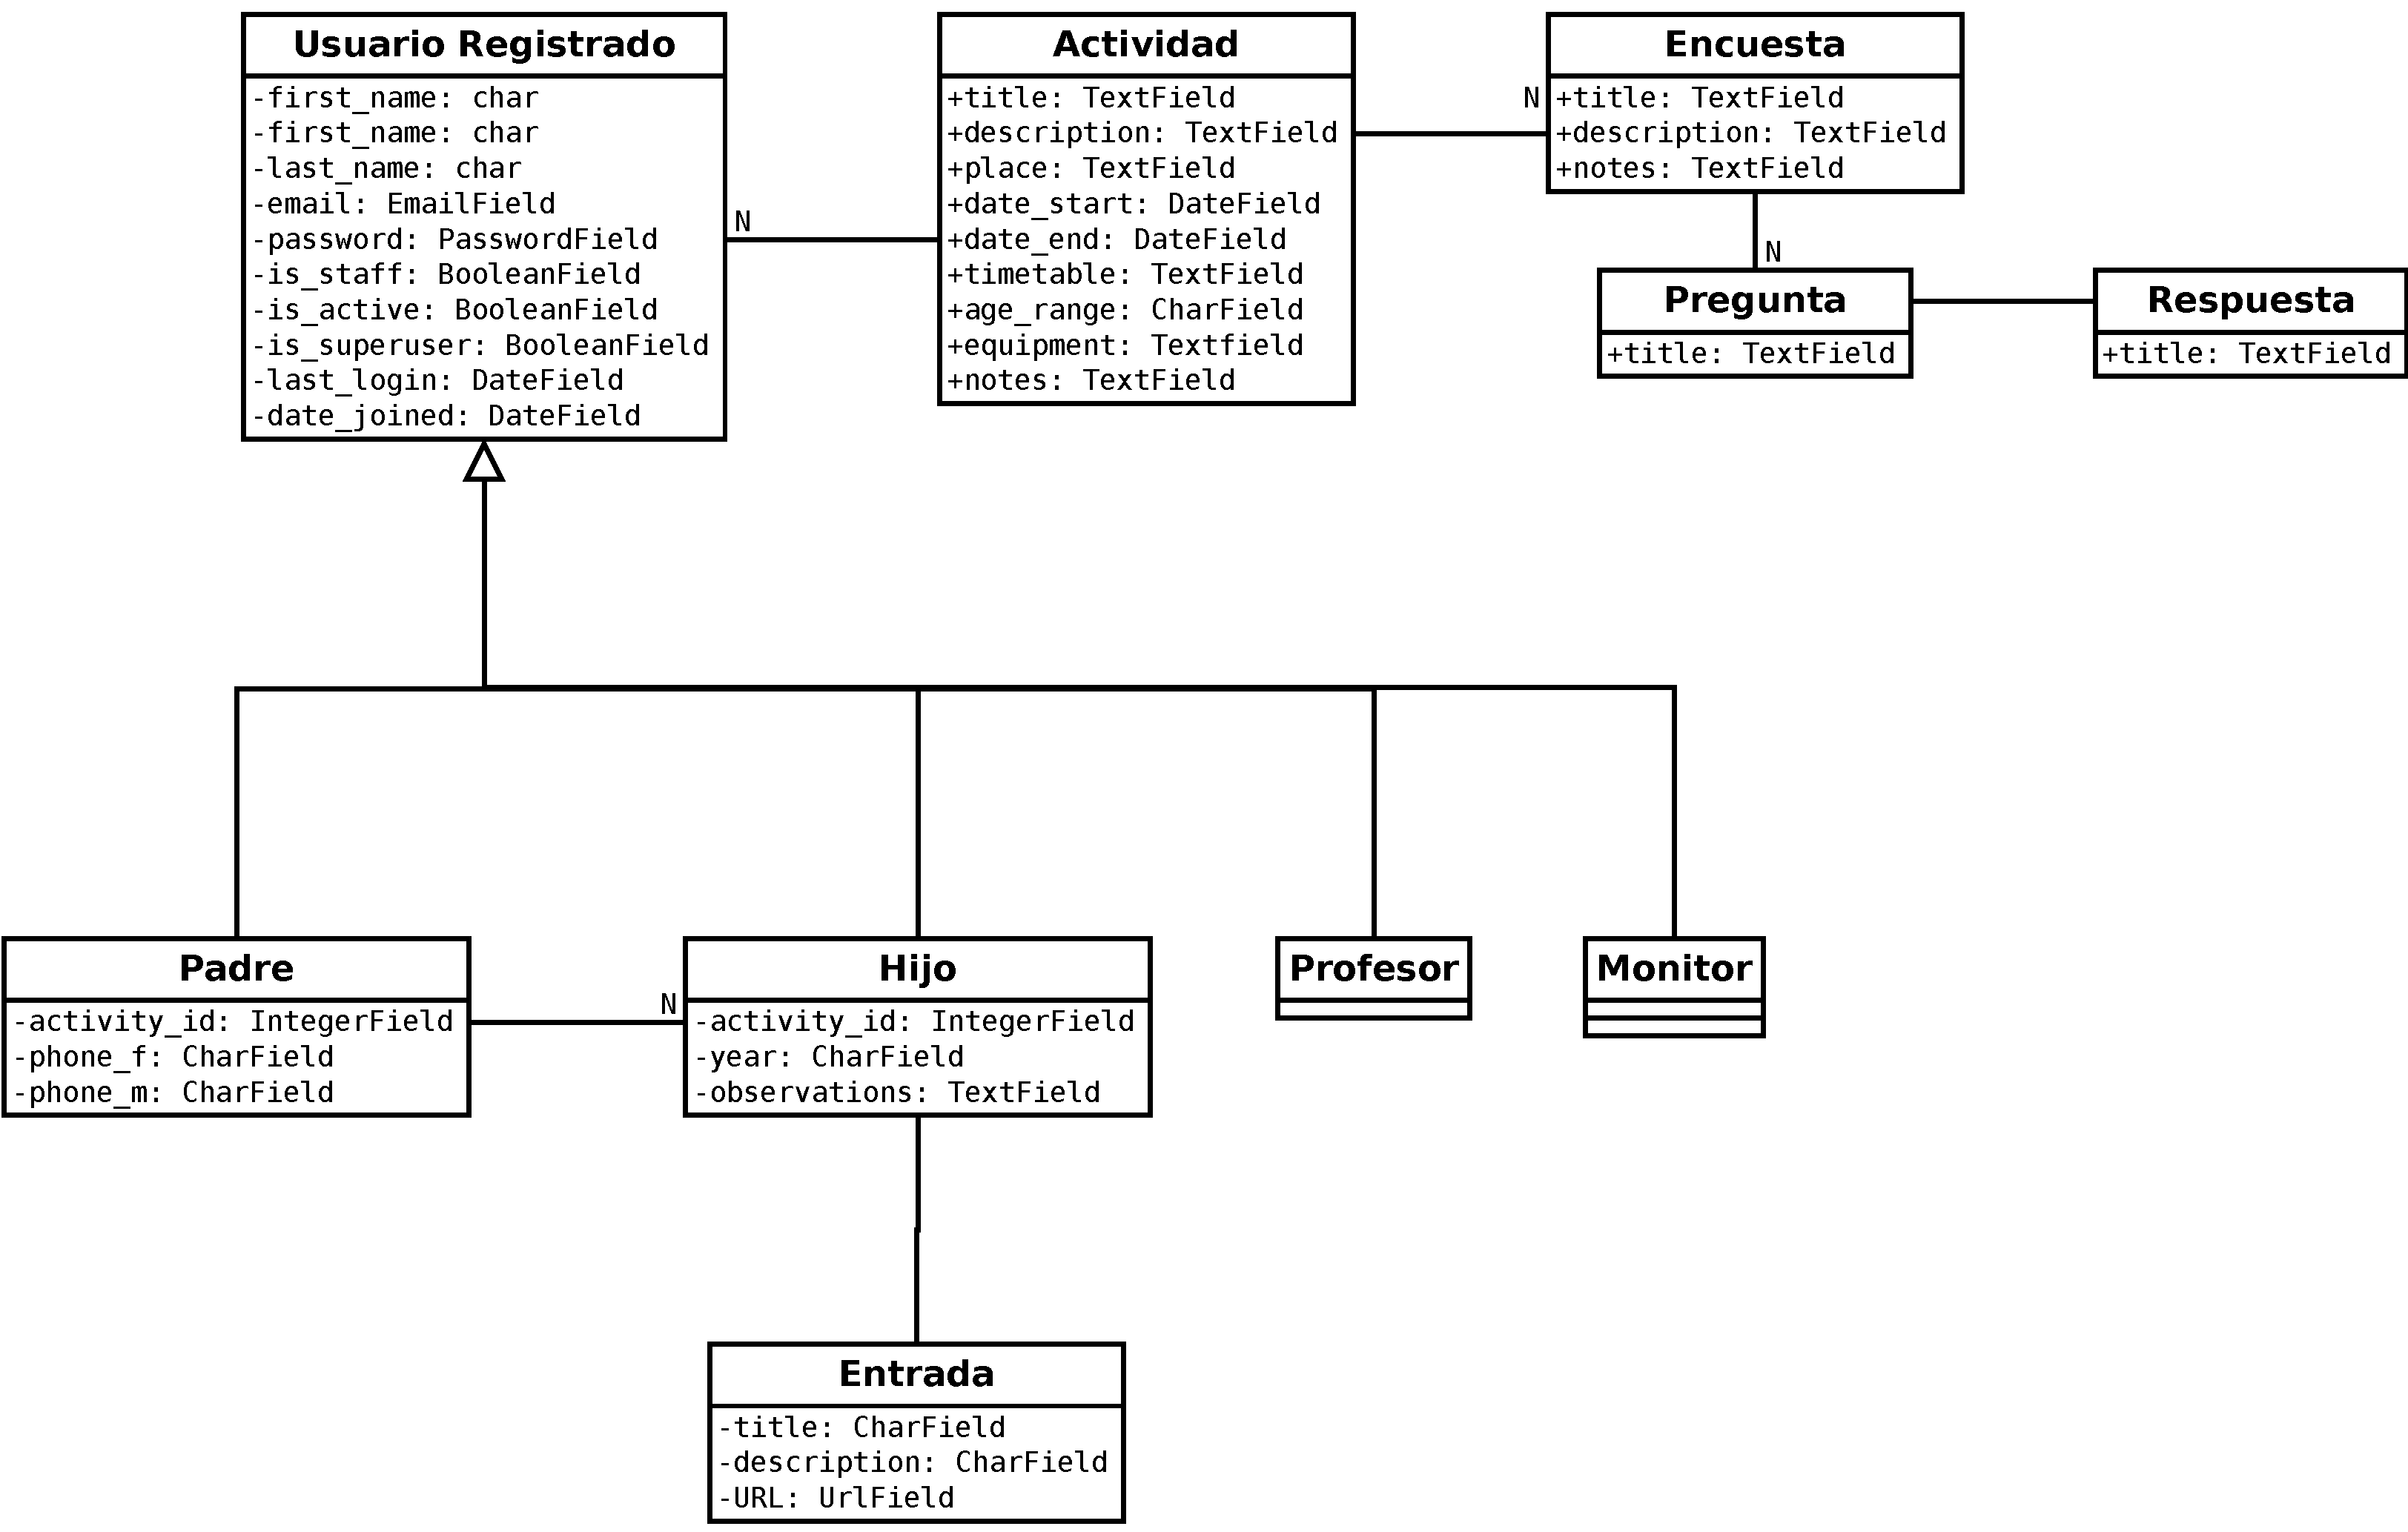
\includegraphics[scale=0.3, keepaspectratio=true]{./Imagenes/Varias/ModeloConceptual.pdf}
			\end{center}
		\end{figure}
		Este modelo 
% 		\end{landscape}

% 		\begin{figure}[!ht]
% 			\begin{center}
% 				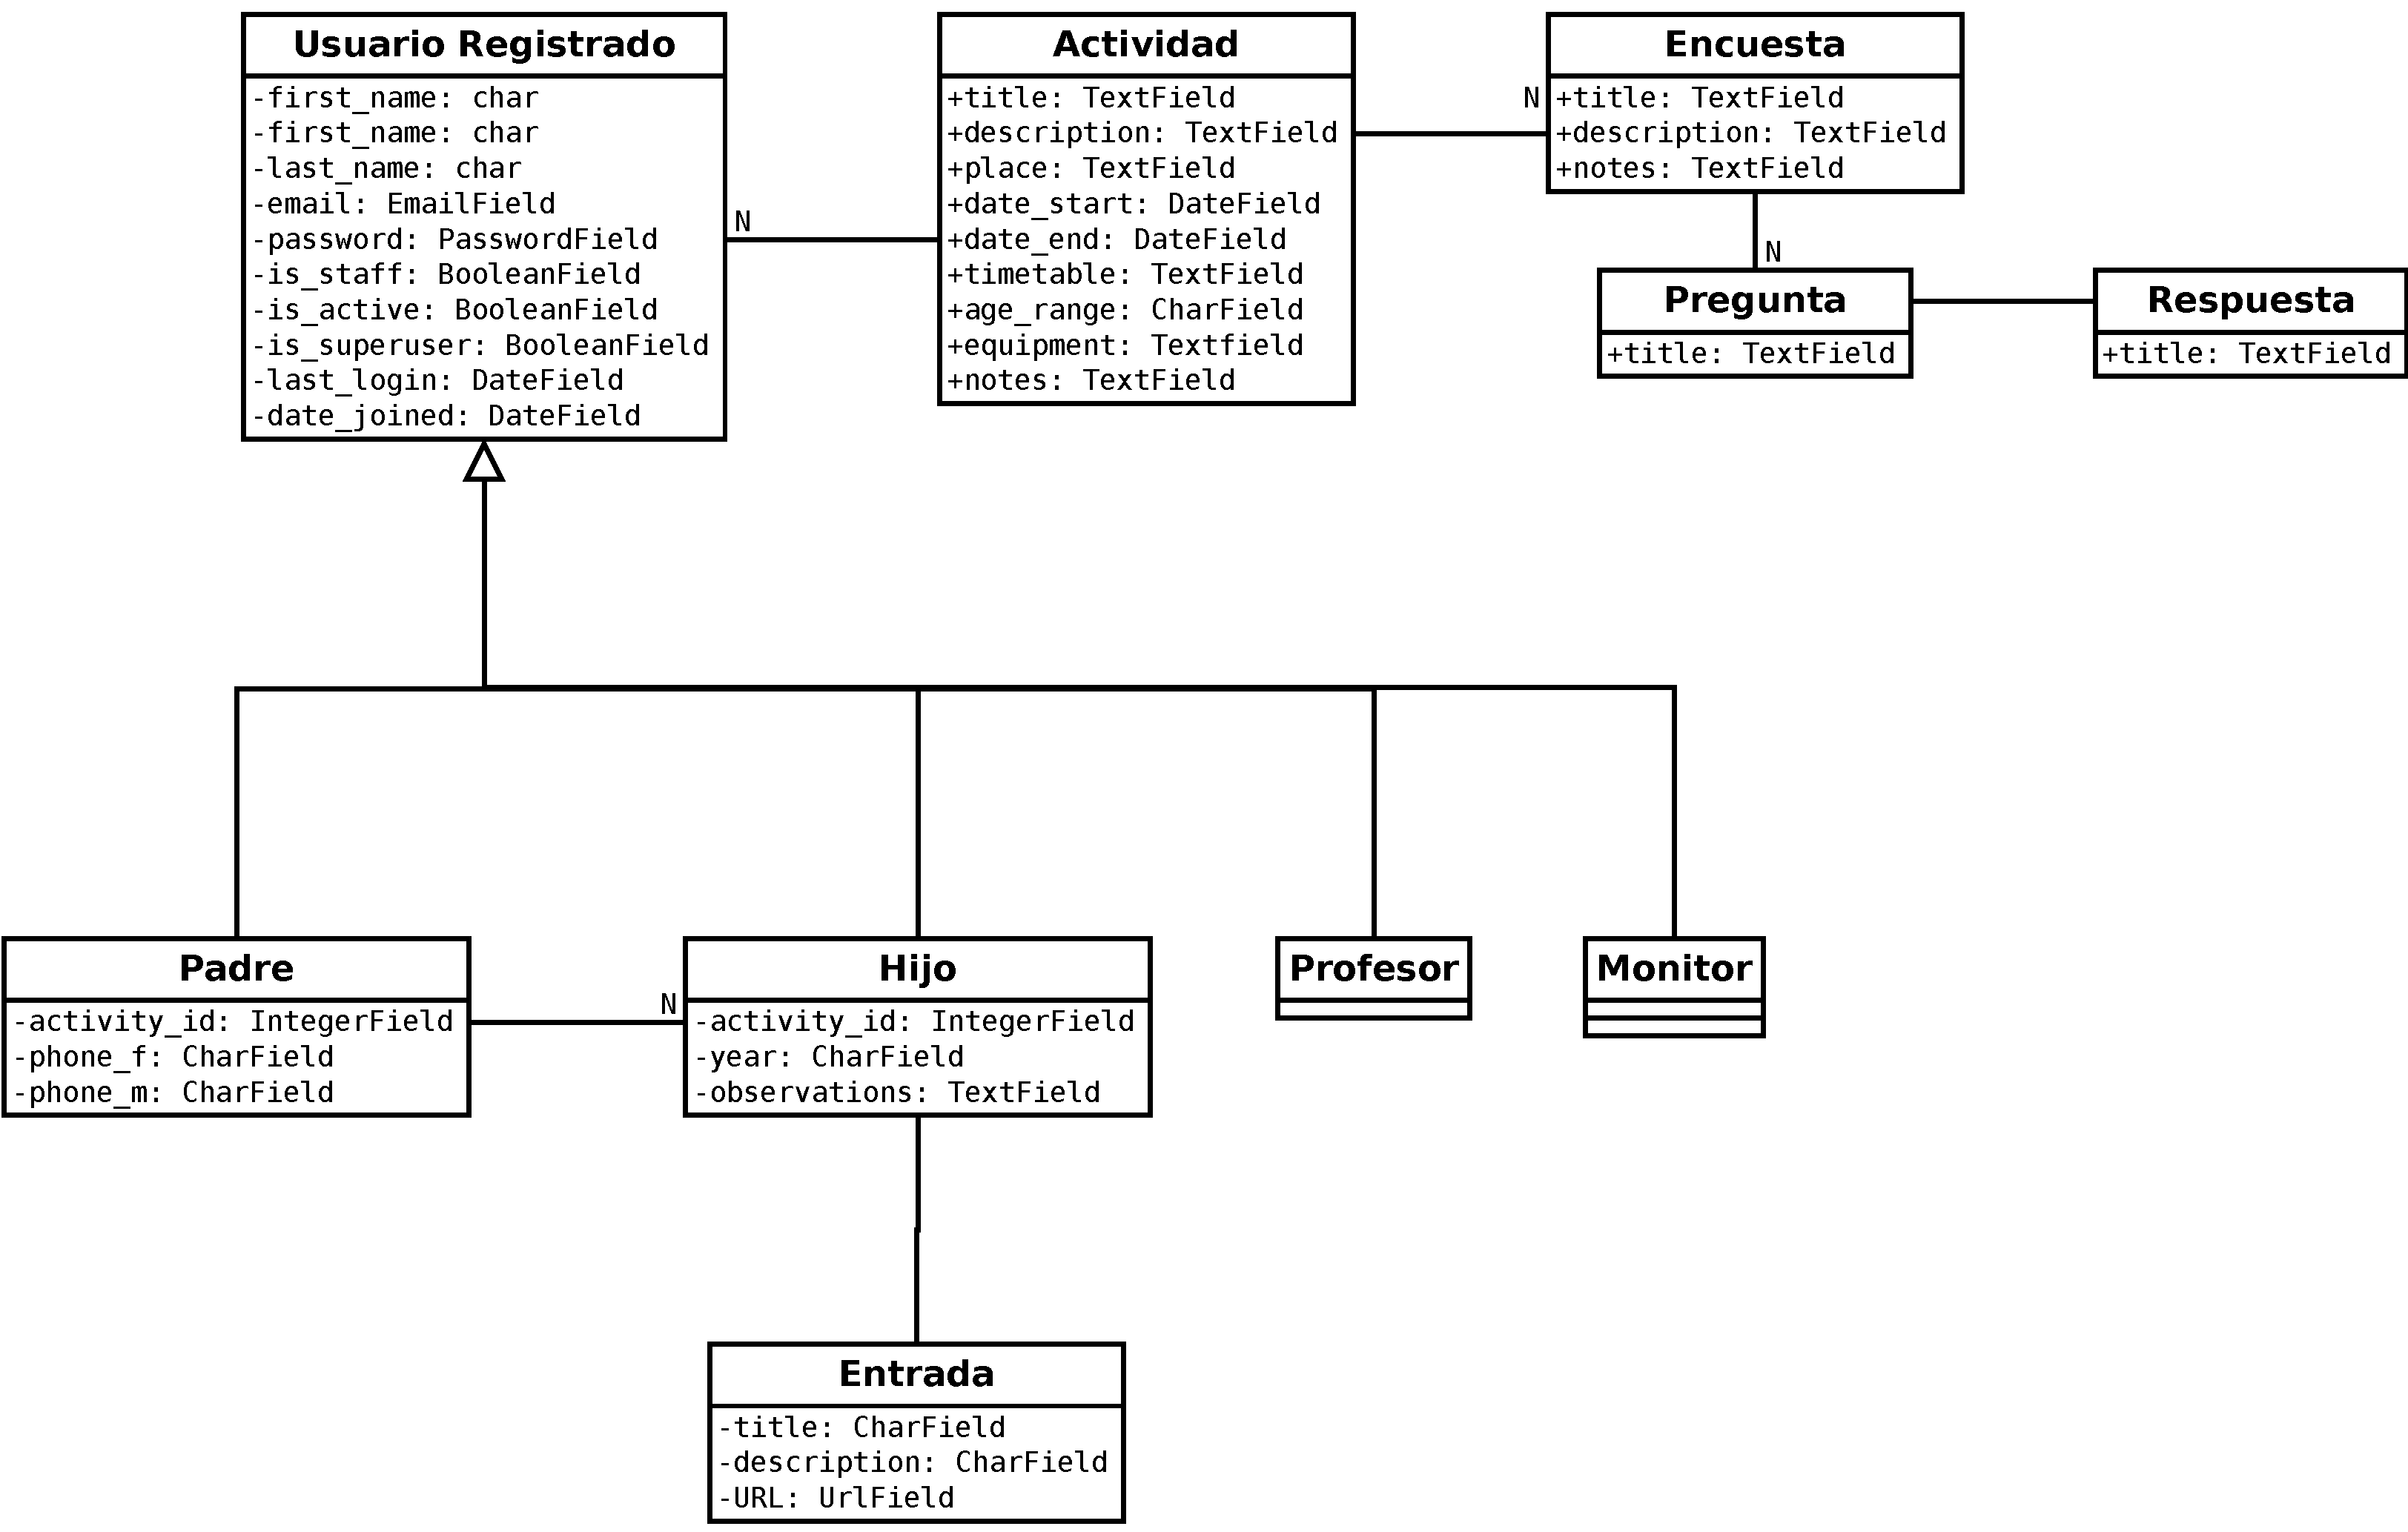
\includegraphics[scale=0.4, keepaspectratio=true]{./Imagenes/Varias/ModeloConceptual.pdf}
% 			\end{center}
% 		\end{figure}
	\newpage
	
	\section{¿Cómo se usa?} \label{como_se_usa}
	\newpage
	
	\section{Referencias} \label{referencias}
	\newpage


	\section{Licencia}
		\begin{center}
			\href{http://creativecommons.org/licenses/by-nc-sa/3.0/es/}{
\includegraphics[scale=0.7, keepaspectratio=true]{./Imagenes/Licencia/licencia.pdf}}
		\end{center}
\end{document}
